% REMEMBER: You must not plagiarise anything in your report. Be extremely careful.

\documentclass{l4proj}

    
%
% put any additional packages here
%

\begin{document}

%==============================================================================
%% METADATA
\title{Green-Workplace: Integrated Web and Mobile application to manage and record commuting carbon footprint via transport mode detection.}
\author{Prith Manickam}
\date{February 05, 2024}

\maketitle

%==============================================================================
%% ABSTRACT
\begin{abstract}
    (need to add)
    Every abstract follows a similar pattern. Motivate; set aims; describe work; explain results.
    \vskip 0.5em
    ``XYZ is bad. This project investigated ABC to determine if it was better. 
    ABC used XXX and YYY to implement ZZZ. This is particularly interesting as XXX and YYY have
    never been used together. It was found that  
    ABC was 20\% better than XYZ, though it caused rabies in half of subjects.''
\end{abstract}

%==============================================================================

% EDUCATION REUSE CONSENT FORM
% If you consent to your project being shown to future students for educational purposes
% then insert your name and the date below to  sign the education use form that appears in the front of the document. 
% You must explicitly give consent if you wish to do so.
% If you sign, your project may be included in the Hall of Fame if it scores particularly highly.
%
% Please note that you are under no obligation to sign 
% this declaration, but doing so would help future students.
%
%\def\consentname {My Name} % your full name
%\def\consentdate {20 March 2018} % the date you agree
%
\educationalconsent


%==============================================================================
\tableofcontents

%==============================================================================
%% Notes on formatting
%==============================================================================
% The first page, abstract and table of contents are numbered using Roman numerals and are not
% included in the page count. 
%
% From now on pages are numbered
% using Arabic numerals. Therefore, immediately after the first call to \chapter we need the call
% \pagenumbering{arabic} and this should be called once only in the document. 
%
% The first Chapter should then be on page 1. You are allowed 40 pages for a 40 credit project and 20 pages for a 
% 20 credit report. This includes everything numbered in Arabic numerals (excluding front matter) up
% to but excluding the appendices and bibliography.
%
% You must not alter text size (it is currently 10pt) or alter margins or spacing.
%
%
%==================================================================================================================================
%
% IMPORTANT
% The chapter headings here are **suggestions**. You don't have to follow this model if
% it doesn't fit your project. Every project should have an introduction and conclusion,
% however. 
%
%==================================================================================================================================


\chapter{Introduction}


\section{Guidance}

\textbf{Motivate} first, then state the general problem clearly. 

\section{Writing guidance}
\subsection{Who is the reader?}

This is the key question for any writing. Your reader:

\begin{itemize}
    \item
    is a trained computer scientist: \emph{don't explain basics}.
    \item
    has limited time: \emph{keep on topic}.
    \item
    has no idea why anyone would want to do this: \emph{motivate clearly}
    \item
    might not know \emph{anything} about your project in particular:
    \emph{explain your project}.
    \item
    but might know precise details and check them: \emph{be precise and
    strive for accuracy.}
    \item
    doesn't know or care about you: \emph{personal discussions are
    irrelevant}.
\end{itemize}

\subsection{References and style guides}
There are many style guides on good English writing. You don't need to
read these, but they will improve how you write.

\begin{itemize}
    \item
    \emph{How to write a great research paper} \cite{Pey17} (\textbf{recommended}, even though you aren't writing a research paper)
    \item
    \emph{How to Write with Style} \cite{Von80}. Short and easy to read. Available online.
    \item
    \emph{Style: The Basics of Clarity and Grace} \cite{Wil09} A very popular modern English style guide.
    \item
    \emph{Politics and the English Language} \cite{Orw68}  A famous essay on effective, clear writing in English.
    \item
    \emph{The Elements of Style} \cite{StrWhi07} Outdated, and American, but a classic.
    \item
    \emph{The Sense of Style} \cite{Pin15} Excellent, though quite in-depth.
\end{itemize}

\subsubsection{Citation styles}

\begin{itemize}
\item If you are referring to a reference as a noun, then cite it as: ``\citet{Orw68} discusses the role of language in political thought.''
\item If you are referring implicitly to references, use: ``There are many good books on writing \citep{Orw68, Wil09, Pin15}.''
\end{itemize}
\subsection{Plagiarism warning}

\begin{highlight_title}{WARNING}
    
    If you include material from other sources without full and correct attribution, you are commiting plagiarism. The penalties for plagiarism are severe.
    Quote any included text and cite it correctly. Cite all images, figures, etc. clearly in the caption of the figure.
\end{highlight_title}


(will remove guidance etc later, keeping it for reference)

% reset page numbering. Don't remove this!
\pagenumbering{arabic} 

\section{Motivation}

Climate change is recognised as one of the most critical global challenges of our time, resulting in a range of negative impacts including rising average temperatures, escalating sea levels, and an increase in extreme weather events (cite). In response, the United Nations' Sustainable Development Goal 13 focuses on climate action, aiming to combat these detrimental effects (cite). A less spoken topic is addressing the large role commuting plays in overall carbon emissions. According to the United States Environmental Protection Agency, transportation accounts for about 29\% of total U.S. greenhouse gas emissions, with a significant portion stemming from daily commuting practices (cite). This statistic underscores the importance of discussing, monitoring, and recording commuting habits in the workplace as a vital step toward reducing overall carbon emissions.

An opportunity to reduce commuting carbon footprint is through hybrid working models, a mix of remote work with traditional office-based work, which was popularised post-pandemic. Moreover, the benefits of remote working benefits range from better employee well-being to reduced overhead costs for companies (cite). However, the importance of working in person is highlighted when considering principles from the Agile Manifesto, which advocates that "the most efficient and effective method of conveying information to and within a development team is face-to-face conversation” (cite). Therefore, there’s a need for teams to discuss their hybrid working schedules to find a balance.

Reflecting the escalating urgency to combat climate change, organisations are increasingly required to integrate comprehensive climate-related disclosures into their reporting practices. Under the International Financial Reporting Standards (IFRS S2) issued by the International Sustainability Standards Board (ISSB) in June 2023, companies are now mandated to provide comprehensive climate-related disclosures, including the indirect greenhouse gas emissions stemming from employee commutes (cite). Additionally, insights into the frequency of in-office attendance are crucial, especially given that a significant 37\% of companies are contemplating office space reallocation to optimise expenses in response to the evolving hybrid work culture. As a result, companies need a tool to record their commuting emissions and patterns.

To effectively follow the mandate, it is imperative to accurately record the commuting carbon footprint of employees. Carbon footprint is the total amount of greenhouse gases generated by an entity (cite). However, such tracking presents challenges due to travel journey variability and the mix of transportation modes. While research on detecting transport modes has been continually pursued, its application to calculate carbon emissions is still in its early stages. As a result, advanced tools capable of detecting transport modes and travel journeys are essential for organisations to meet climate-related disclosure mandates like the IFRS S2. 

Despite the clear need, the market currently lacks a comprehensive platform that effectively allows employees in a company to discuss, monitor, and record their carbon footprint. Such a platform is not merely an operational tool but a strategic asset, empowering companies to make informed decisions that do not compromise workplace efficiency and mitigate the effects of climate change.

\section{Aim}

The objective is to create an integrated Web and Mobile app, Green-Workplace, for companies to manage and record employees' carbon footprint. Specifically for the web app, employees can chat and vote with their team(s) to set their hybrid work schedules. Provide web solutions to record their carbon footprint. In addition, monitor this data in dashboards at an individual, team, and company level.

The mobile application aims to accurately track users' travel journeys and calculate their carbon footprint by employing supervised machine learning for transport mode classification. This is achieved by harnessing users' GPS and motion sensor data. The effectiveness of the project in discussing, monitoring, and recording hybrid working days and commuting carbon footprint will be experimentally validated.



%==================================================================================================================================
\chapter{Background}


What did other people do, and how is it relevant to what you want to do?
\section{Guidance}
\begin{itemize}    
    \item
      Don't give a laundry list of references.
    \item
      Tie everything you say to your problem.
    \item
      Present an argument.
    \item Think critically; weigh up the contribution of the background and put it in context.    
    \item
      \textbf{Don't write a tutorial}; provide background and cite
      references for further information.
\end{itemize}


Due to the lack of systems in the market that facilitate employees in organisations to communicate, monitor and record commuting carbon footprint, the analysis will be divided into three main areas: First, the research will involve an exploration of existing platforms that enable team communication and decision making to set hybrid working days. Second, applications that display carbon footprint analytics can be viewed at an individual, team, and company level. Third, an examination of applications and literature to help calculate users’ carbon footprint will be conducted. This section provides a review of several of these products, identifying any strengths or weaknesses and discussing how each has influenced the design and development of Green-Workplace.

\section{Current Systems for Team Communication and Decision Making (Microsoft Teams)}

\begin{figure}[ht]
  \centering
  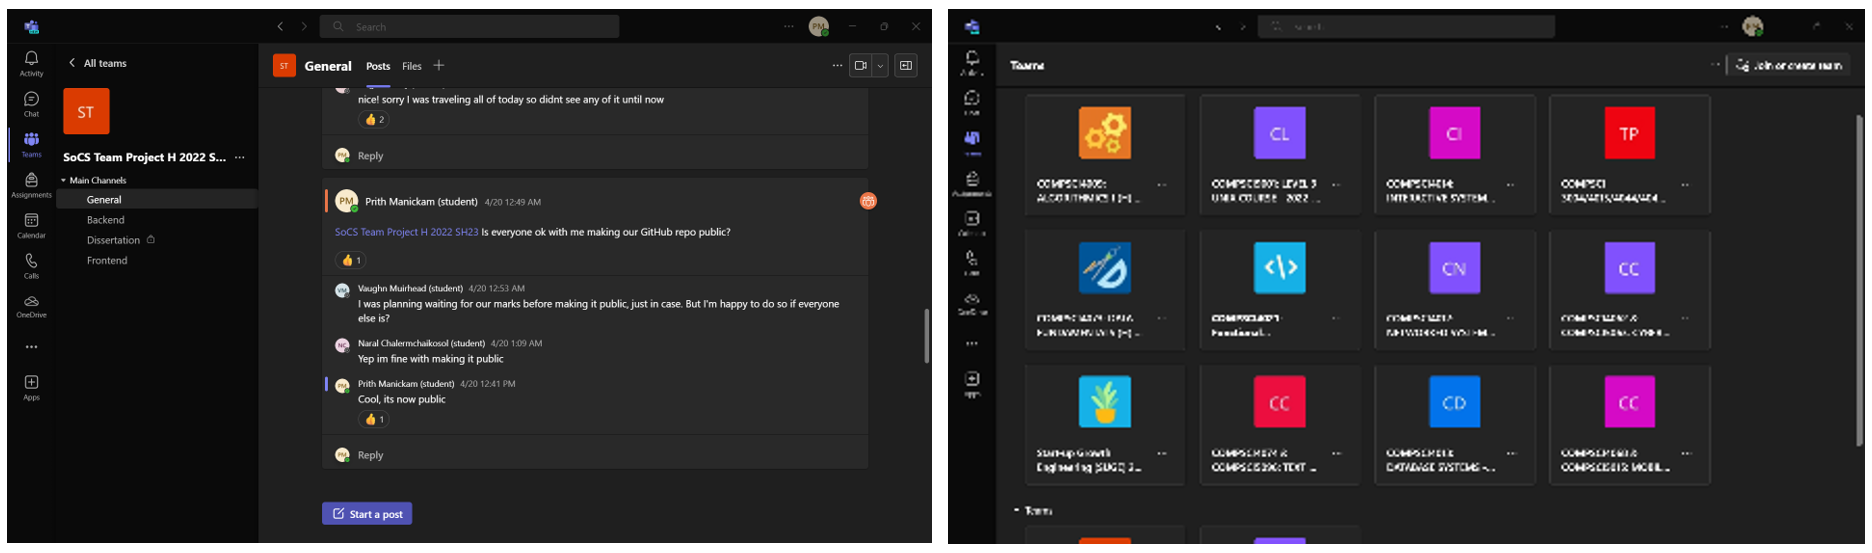
\includegraphics[width=\linewidth]{images/MSTeams.png}
  \caption{MSTeams Team Channel.}
  \label{fig:msteams}
\end{figure}

The rationale for analysing systems that connects team members serves as the foundation for monitoring and recording carbon footprint. In examining current systems for team communication and decision-making, several platforms were considered, including Slack, Google Meet, and Zoom. However, Microsoft Teams (MS Teams) emerges as the most prominent and effective app, especially in the context of discussing hybrid work schedules. MS Teams offers comprehensive functionality that enables team members to both chat and vote, making it a representative model to analyse for contemporary communication systems.

A strength that saves employees time for manual joining is that administrators can effectively structure organisations through the creation and management of users and teams by using the MS Teams Admin Center. MS Teams' major strength is its team communication features offering team chat, voice, and video conferencing. In terms of decision-making, MS Teams has a polling tool to allow team members to vote for work at office days, where the table can be pinned for continuous reference. Green-Workplace can harness administrative roles by using admin accounts and employee team owner roles to populate and structure their organisation. For the context of discussing work on office days, messaging chat and toggling between teams can be sufficient for Green-Workplace. 
    
\section{Current systems for commuting carbon footprint analytics dashboard}

\subsection{CBN EXPERT by CBN Expert Ltd}

\begin{figure}[ht]
  \centering
  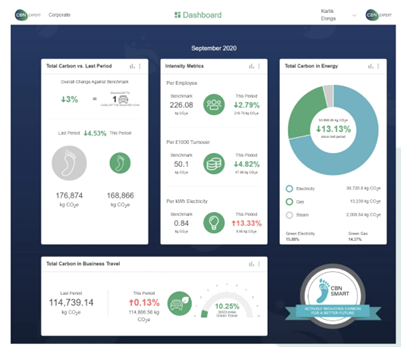
\includegraphics[width=0.75\linewidth]{images/CBN Expert.png}
  \caption{CBN EXPERT dashboard.}
  \label{fig:transportmodedetection}
\end{figure}
 
CBN EXPERT is Carbon Accounting Software that collates, measures, tracks, and reports the carbon emissions across a business. The strength of the dashboard where the design is icon-based to make it more intuitive to understand. It also gives a visualisation by quantifying how much carbon emissions have been saved e.g. 2 cars off the road per year. Another strength of the dashboard is that you can measure your current metric against your set benchmark or the last period/month where the carbon footprint icon decreases in size and turns green if it is below it. The drawback of this site is that you can only see the dashboard on a company level and not also from a team or individual level. Additionally, whilst it compares to last month it doesn’t show progress from the last couple of months or weekly. Green-workplace can leverage the using colour indications to compare individual, team, and company metrics against set company standards. Visualisation can be used to compare carbon footprint to the number of trees to offset it. Additionally, historical trends of carbon footprint can be displayed via line charts.


\subsection{WeSpire}

\begin{figure}[ht]
  \centering
  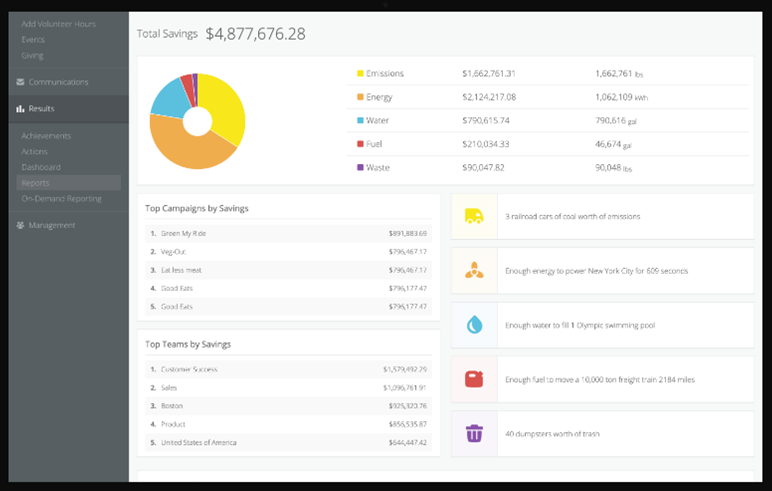
\includegraphics[width=0.75\linewidth]{images/WeSpire.png}
  \caption{WeSpire dashboard.}
  \label{fig:wespire}
\end{figure}
 
‘WeSpire’ provides a platform for employee engagement in sustainability and social responsibility. The benefits of visualisation and icons like with CBN EXPERT also apply to this product. A unique benefit of this platform is that it contains gamification elements such as leaderboards to compare performance among teams, individuals, or campaigns within an organisation. This gamified aspect serves as a motivational tool to encourage sustainable practices. The drawback of the leaderboard for teams is that it lacks further detail for context such as the number of employees, and its division. Furthermore, it lacks the functionality to sort or search for a particular team. 

\section{Current systems and Literature to record commuting carbon footprint}

\subsection{Carbon Footprint Calculator by Carbon Footprint Ltd.}

\begin{figure}[ht]
  \centering
  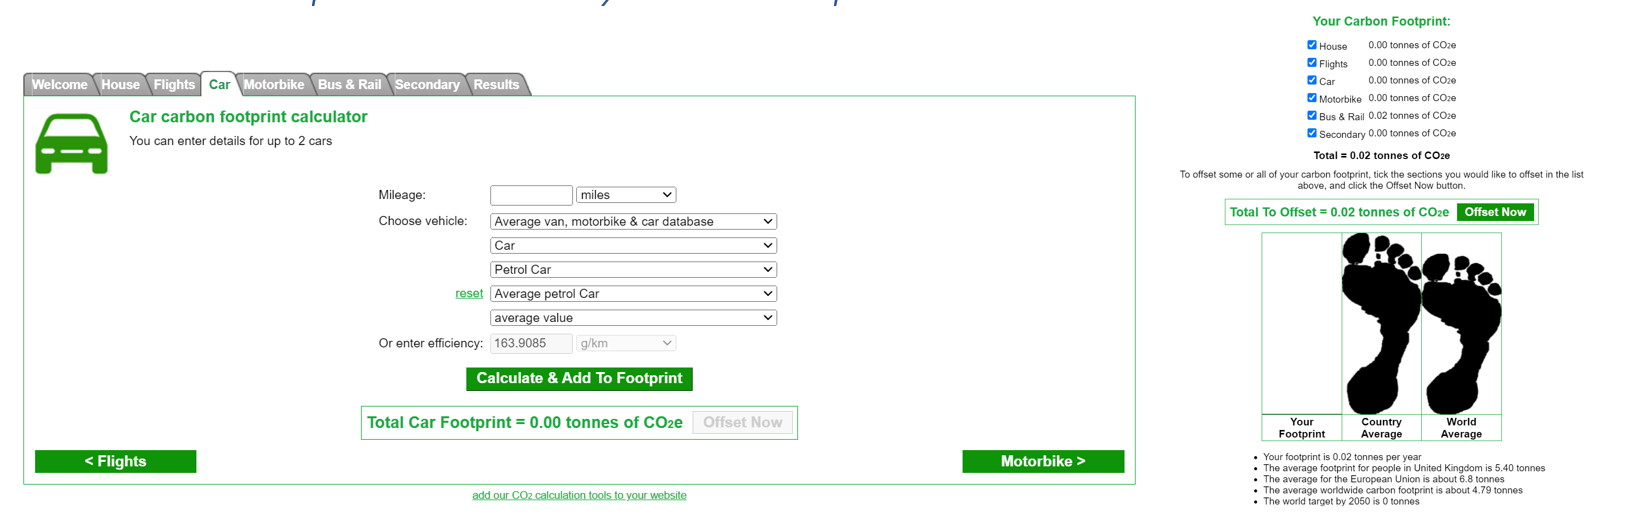
\includegraphics[width=\linewidth]{images/carbon footprint calculator.png}
  \caption{Carbon footprint calculator website.}
  \label{fig:carbonfootprintcalculator}
\end{figure}
   
Carbon Footprint Calculator is a tool designed for individuals to input various data related to their lifestyle, including transportation, home energy use, and more, to calculate the total carbon emissions. It is comprehensive taking into account various factors for car transport to give an accurate carbon footprint value. It allows you to cumulatively add transports for your journeys and give total value. The drawback of this calculator is the assumption all users know the distance they travelled on transports without a visible odometer such as a train, and no option to choose duration instead. Whilst using distance would be more accurate, there is no functionality that could help find the distance for the user. Additionally, the website design and layout could improved to be more appealing. Green-Workplace would ensure users have an option to set a duration and add transport parameters e.g. car engine type and number of passengers, to increase calculation accuracy of carbon footprint.

\subsection{Transport Mode Detection Literature Review.}

Transport Mode Detection (TMD) is an emerging area that has gained significant attention in recent years, primarily due to its potential to facilitate intelligent transportation systems, urban planning, and environmental monitoring. TMD systems aim to accurately identify the mode of transport (e.g., walking, cycling, driving) based on various data sources, including but not limited to GPS, accelerometer data, and even contextual information (cite). The significance of TMD systems is underscored in the context of assessing the commuting carbon footprint as the mode of transportation plays a critical role in determining the volume of carbon emissions. By accurately capturing the distance traveled and integrating it with the mode of transport, TMD systems facilitate precise calculations of an individual's or a community's commuting carbon footprint
Most literature on TMD systems relies on Classifier Machine Learning (ML) algorithms which follow four main steps of data collection, preprocessing, feature extraction, and classification (cite). However, there is limited literature where the system is deployed in a real-world application and users validate the accuracy of the classifications in real-time and collate received information into a journey. The two pivotal areas in the research and practical application of TMD systems are increasing the accuracy of TMD systems and reducing device battery consumption.

The literature on Transport Mode Detection highlights the integration of diverse data sources to enhance transport mode identification accuracy. Prominently, GPS, accelerometers, and gyroscopes are among the most utilised due to their reliability and the rich movement data they provide (cite). However, studies have also delved into the potential of sound as a data source to offer valuable context-specific information. However, a challenge would be the distortion of sound-based data in the presence of multiple commuters, which can lead to ambiguous interpretations of the surroundings (cite). Similarly, with magnetometers, it's found that magnetic fields can be distorted by nearby ferromagnetic materials, such as steel in cars and buildings, which can lead to inaccurate readings (cite). To counter these limitations, recent trends in TMD emphasise the importance of integrating contextual factors, including the time of day, weather, and urban structure, to significantly refine detection accuracy and overcome the shortcomings of individual data sources (cite).

TMD research underscores a crucial trade-off between detection accuracy and battery life. Higher GPS and sensor data sampling rates enhance accuracy, capturing detailed transport mode transitions and tracking nuances like vehicle turns. However, GPS's intensive power use, due to constant satellite communication and complex location computations, leads to rapid battery drain, compromising app usability (cite). To counter this, one solution called FogTMDetector' by Kamalian and Ferreira aims for a balance. It samples sensor data every 1 second and GPS data every 10 seconds, optimising accuracy while managing battery consumption. Additionally, it conserves power by sending data to the backend every 90 seconds, showcasing a strategic approach to maintain both precision and efficiency in TMD systems (cite).


%==================================================================================================================================
\chapter{Requirements Gathering}
What is the problem that you want to solve, and how did you arrive at it?
\section{Guidance}
Make it clear how you derived the constrained form of your problem via a clear and logical process. 


\section{Requirement Elicitation}

\subsection{User Scenarios}

Multiple user scenarios were developed, describing how different types of users may interact with the system, including company administrators, team members, and team owners. Several user scenarios have been crafted, detailing the interaction patterns of various user categories with the system. These categories encompass system administrators, team members, and team owners, ensuring a comprehensive understanding of user-system engagement. (reference)

\begin{itemize}
    \item Jordan is a Company Admin for his X company on Green-Workplace. Jordan is responsible for managing the company's structural dynamics and ensuring that sustainability goals are integrated into every team's workflow. Jordan receives information from HR on employees who have joined or left the company, as well as teams (with the team member taking on the role as a team owner) that added or removed. Jordan navigates to the ‘Employee Management’ section, where he sends out personalized email invites to these new employees, and then deletes the accounts of employees who have left. Jordan then navigates to the ‘Team Management’ Section to create a team, designating a team owner, optionally adding team members, then looking at existing teams and deleting the ones that are no longer in the company. Upon receiving information from regulators or the company sustainability team that carbon standards need to be changed, the company sets a new green,  amber, and red carbon standard visible to all employees.
    \item Ben is a Team Member in the ‘Frontend Dev’ and ‘UI/UX’ teams in Company X. Ben receives an email from the Company Admin with a link to create an account for Green Workplace. Once he has he can set his preferences for the days he wants to go to the office for both teams. He types into his team chat on his justification of his work at office days preferences, and discusses with his team to reach a consensus on what the teams should be. He could set his carbon footprint by Manually entering the transport journey or the Google Maps Page but chooses to set it using the mobile app as recommended. Before Ben leaves his house, he opens the app and presses start and once he reaches his office he presses stop. Ben manually edited one of the automatically added transport entries, as it mis-detected Bus instead of Car. Ben split his carbon footprint value 50\% for both teams as he spent an equal amount of time working for each team on that day. Ben reviews his individual, team, and company dashboard to how it compares to the company carbon standard and how it has progressed in the last 4 weeks. Ben decides to fix the fix incorrect spelling of his last name and change his password to be more secure on the accounts page.
    \item Emma is a Team Owner of the ‘Frontend Dev’ team in Company X. She can perform functions like a Team Member but has extra functionality. She adds a new team member and removes an existing team member that joined another team. After discussion with the team members in the team chat and looking at the work at office preferences, she sets the team office Days as Tuesday and Thursday. After talking to the higher management, she decides to change the team name to ‘Product 1 Frontend Dev’.
\end{itemize}

These scenarios were then converted into user stories, to allow a more high-level, detailed description of the requirements.

\subsection{User Stories}
\textbf{Admin}
\begin{itemize}
    \item As a Company Admin, I want to be able to send emails to employees so that they can register for the app.
    \item As a Company Admin, I want to be able to add and delete teams, so that I can adapt the company's structure.
    \item As a Company Admin, I want the ability to set the company's carbon standard, so that I can establish clear sustainability targets for the entire organization.
    \item As a Company Admin, I want to view all teams connected to the company (from the company dashboard) and sort them based on carbon emissions, so that I can assess each team's contribution to the company's carbon footprint.
\end{itemize}

\textbf{Team Member}
\begin{itemize}
    \item As a Team Member, I want to register from the invitation link sent by my company admin and login to my account, so that I can personalise my Green-Workplace experience.
    \item As a Team Member, I want to set my carbon footprint using the web app from Google Maps or Manually Add page, so that I can get a good estimate of my carbon footprint of my commutes.
    \item As a Team Member, I want to set my carbon footprint using the Mobile App from the start and end of my journey, so I can get a further accurate carbon footprint of my commutes.
    \item As a Team Member, I want to view my individual dashboard, so that I can view my individual carbon metrics to understand how my weekly choices affect carbon emissions.
    \item As a Team Member, I want to be able to engage in real-time chat with my team members, so that I can discuss changes to work at office days and collectively reduce commuting carbon footprint.
    \item As a Team Member, I want to view the Team Dashboard, so that I can see what is set for WAO days and also assess our team's environmental performance.
    \item As a Team Member, I want to view the Company Dashboard, so that I can see the company's collective carbon metrics, a list of all teams carbon footprint, and assess our companies environmental performance.
    \item As a Team Member, I can change my password in the accounts page, if I want to create a stronger password.
\end{itemize}

\textbf{Team Owner}
\begin{itemize}
    \item As a Team Owner, I want to have all the capabilities of a Team Member plus additional administrative privileges, so that I can record data alongside my team.
    \item As a Team Owner, I want to set my team's work at office days after discussion in team chat so that team members can be reminded what days to come into the office.
    \item As a Team Owner, I can add and remove team members from my team within the company, so that I could add newly joined members or remove the ones that left.
    \item As a Team Owner, I can edit the team name of our team so that it displays the new name required by the organization.
\end{itemize}

\section{Functional Requirements}

After completing the requirement elicitation process, a set of functional requirements was defined. These requirements serve as a continuous reference point throughout the project to guarantee that the system fulfills all its initial criteria. The MoSCoW method (cite) was employed for prioritization, categorizing requirements into one of the following labels:

\begin{itemize}
    \item \textbf{Must Have}: Describes requirements that are critical to the success of the project, where failing to meet these will result in a solution that is not viable.
    \item \textbf{Should Have}: Describes requirements that are important, but the success of the project does not depend on their completion.
    \item \textbf{Could Have}: Describes requirements that are desirable, but would be acceptable if they were not present in the final system.
    \item \textbf{Won’t Have This Time}: Describes requirements that will not be delivered, but are useful to state in order to make clear the scope of the project.
\end{itemize}

Similarly, with the user stories in Section 3.1.2, the functional requirements have been separated into user types so that throughout development a single user type could be focused on at one time. As team owners should have access to similar functionalities as team members, these two user types have been joined into a Green-Workplace User type. Requirements are listed below, along with their importance, represented by MH, SH, CH, or WH, which corresponds to the Must Have, Should Have, Could Have, and Won’t Have This Time labels respectively. 

\textbf{Green-Workplace User}
\begin{itemize}
    \item \#1: MH – Users must be able to register to Green-Workplace using the invitation link sent to their inbox.
    \item \#2: MH – Users must be able to view their company dashboard displaying company and team carbon stats.
    \item \#3: CH - Team Members could be able to see a line chart from all dashboards showing carbon footprint stats progression from the last four weeks and months.
    \item \#4: CH - Users could be able to see a line chart from all dashboards showing carbon footprint stats progression from the last four weeks and months.
    \item \#5: SH – Users should have an account page where they can change their name and password.
    \item \#6: CH – Users should be able to use the forgot password page to get sent a link to reset their password.
\end{itemize}

\textbf{Admin}
\begin{itemize}
    \item \#7: MH - Admins must have an Add Employee Page to send emails to employees so that they can register for the app.
    \item \#8: MH - Admins must have a Manage Teams Page where they can create a team, with an assigned Team Owner, and delete a team.
    \item \#9: SH – Admins should be able to set the company’s carbon standard using the Admin Functions Page.
\end{itemize}

\textbf{Team Member}
\begin{itemize}
    \item \#10: MH – Team Members can register to Green-Workplace using the invitation link sent to their inbox.
    \item \#11: MH – Team Members must be able to set their Carbon Footprint Manually.
    \item \#12: SH – Team Members should be able to set their Carbon Footprint using Google Maps API.
    \item \#13: SH – Team Members should be able to set their carbon footprint using the Mobile App via Transport Mode Detection.
    \item \#14: MH – Team Members must be able to view their individual dashboard and set work at office days preference for each team.
    \item \#15: MH – Team Members must be able to view their team dashboard displaying team and individual carbon stats.
    \item \#16: SH – Team Members should be able to use the Team Chat Page to talk with each of their teams in real-time.
    \item \#17: CH – Team Members would be notified in the top navbar if they received a new Team Chat message.
\end{itemize}

\textbf{Team Owner}
\begin{itemize}
    \item \#18: MH – Team Owners must be able to use the Team Ownership Functions Page to officially set the team's work at office days.
    \item \#19: MH – Team Owners must be able to use the Team Ownership Functions Page to add team members from the company, and remove existing team members.
    \item \#20: CH – Team Owners could be able to use the Team Ownership Functions Page to change the name of their team.
\end{itemize}


\section{Non-Functional Requirements}

Along with functional requirements, a set of non-functional requirements was established before any further progress of the project could take place. Whilst functional requirements describe what the system should do, non-functional requirements are equally important as they describe the properties that the system must have (cite). All established non-functional requirements were Must Have requirements, as they are all essential in a successful product.

\begin{itemize}
    \item \#21: MH - The system must be modular, allowing for different services, feeds, and visualisations to be added or removed in the future.
    \item \#22: MH - The application must be responsive and should function correctly on both desktop and mobile devices without any problems or restrictions of features.
    \item \#23: MH - The system must be portable and work on all modern browsers.
    \item \#24: MH - The system must be intuitive and easy to use by untrained users.
    \item \#25: MH - The system must perform well, with quick load and response times, allowing for better a user experience
    \item \#26: CH - The system could have a light and dark mode to cater to user preferences.
\end{itemize}




%==================================================================================================================================
\chapter{Design}
How is this problem to be approached, without reference to specific implementation details? 
\section{Guidance}
Design should cover the abstract design in such a way that someone else might be able to do what you did, but with a different language or library or tool.

\section{System Architecture}

The architecture of Green-Workplace adheres to the three-tier architecture pattern which consists of a presentation layer, an application layer, and a data layer. This architecture pattern is carefully designed to interact seamlessly while maintaining clear boundaries to prevent the propagation of defects across layers. This helps the system's modularity and flexibility, meeting requirement \#21. This architecture lays a solid foundation for future scalability, the addition of new features, and maintenance. This helps the system's modularity and flexibility, meeting requirement \#21.

At the top of the architecture is the Presentation Layer, which includes both the Mobile Client and the Web Client. The Mobile Client is built with React Native and the Web Client uses ReactJS combined with Material-UI (MUI) for responsiveness and to speed up development. This layer is responsible for presenting the user interface, visualizing data, and facilitating user interactions with the system. External services like the Google Maps API are utilised in this layer to display the map and route for the web solution to calculate the carbon footprint.

The Application Layer is the system's logical core, where the NodeJS and Express framework operates as a web server equipped with JWT (JSON Web Tokens) for secure user authentication. This layer is where the application's business logic is processed, including handling requests, and executing the machine learning inference. Additionally, it utilises APIs such as Nodemailer to send out emails and Nodeschedule to weekly record user carbon footprint data. 

The Data Layer serves as the foundation of the application, housing the essential data-related components. At its core is the Relational Database managed by Supabase, which provides a scalable and reliable storage solution. The Trained ML Model, a Random Forest Classifier in JSON format, is integral for the real-time prediction of transport modes based on various mobile sensor data. The efficiency of the Data Layer is significant, as it handles potentially large volumes of diverse transportation data with low latency to support real-time processing needs.


\section{System Architecture}

\subsection{Initial Prototyping}
In the initial phase of prototyping for Green-Workplace, Figma wireframes were created to visualise the user interface and ensure that it aligned with the project's functional requirements. Wireframes, often described as the blueprints of a user interface, serve as a bridge between a site's structural aspects and its visual design (cite). This early visualisation helps in identifying potential usability issues and layout inefficiencies, thus allowing for adjustments before further development. Figma was chosen to speed up the design process through the use of reusable components, ensuring uniformity across the various pages of the app (cite). The design of the pages in Green-Workplace closely adhered to Nielsen’s 10 usability heuristics (UH), ensuring that the interface was user-friendly and intuitive (cite).

\subsection{Company Dashboard}

\begin{figure}[ht]
  \centering
  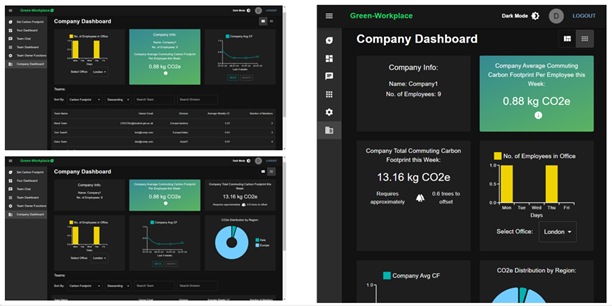
\includegraphics[width=\linewidth]{images/company dashboard.png}
  \caption{Company dashboard page.}
  \label{fig:companydashboard}
\end{figure}

Three specialised dashboards were developed to facilitate the monitoring of carbon footprint data across different levels of granularity: an Individual Dashboard for personal carbon footprint tracking, a Team Dashboard for group metrics, and a Company Dashboard for overarching organisational insights. For the creation of these dashboards, the React library MUI was utilized to implement chart components, ensuring both a high degree of responsiveness to browser dimension changes and the seamless integration of additional components as needed.

The company dashboard clearly shows the summary view by default and offers a detailed view for more in-depth information, helping meet UH\#7 Flexibility and efficiency of use and UH\#1 ‘visibility of system status’. The dashboard displays the summary view by default to focus the important data to the user, achieving UH\#8 aesthetic and minimalist design. To effectively monitor certain teams, divisions, or teams with the highest carbon footprint, the functionality to sort and filter teams based on characteristics according to their preferences helps meet User control \& freedom UH\#3. The dashboard leverages the strength of displaying icons from 2.2.1, where it translates CO2e emissions into the number of trees required to offset these emissions which makes the abstract concept of carbon emissions more tangible and understandable, to match between the system and the real-world UH\#2. Additionally, it utilises a pie chart in the detailed view to monitoring carbon footprint distribution by region. 

The common layout and components such as the line progress chart are shared for each dashboard type which helps to speed up user recognition and understanding which meets \#4 consistency and standards. The team dashboard (Appendix B.2) leverages strengths from gamification in 2.2.2, where it utilises a leaderboard where team members with the lowest carbon footprint appear at the top.

\subsection{Registration}

\begin{figure}[ht]
  \centering
  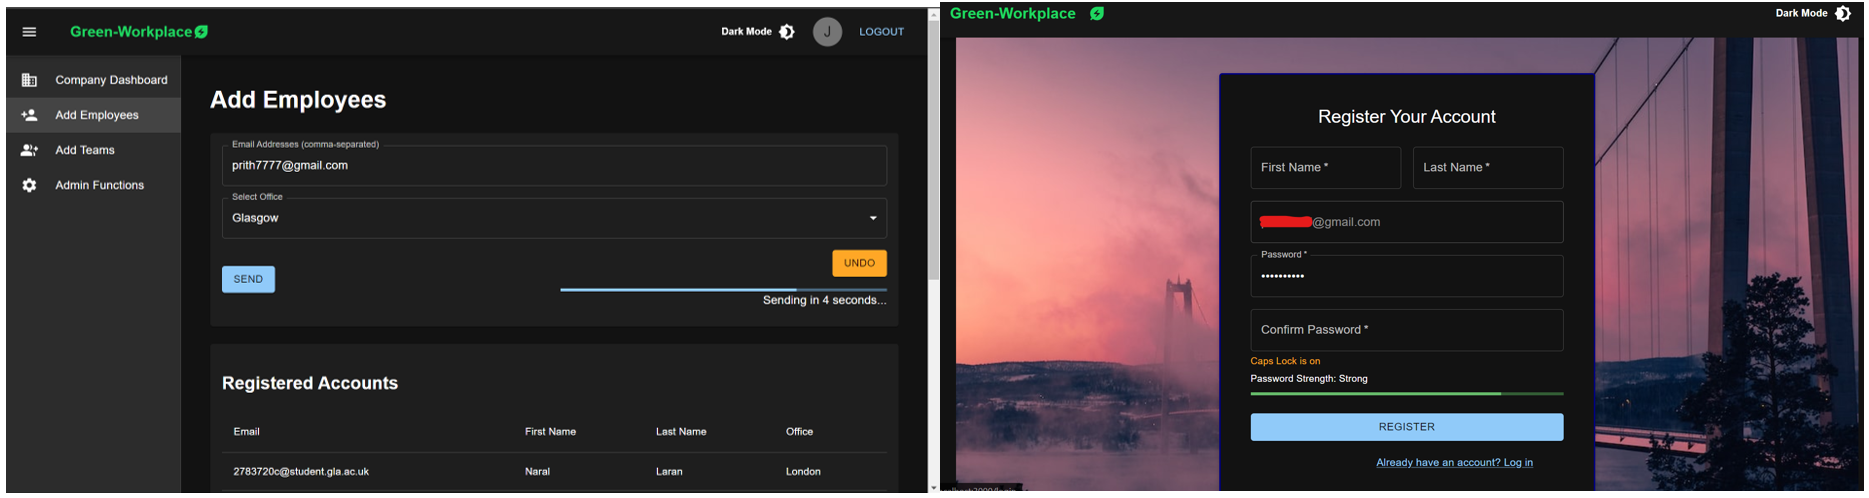
\includegraphics[width=\linewidth]{images/registration.png}
  \caption{Add Employees and Sign up pages.}
  \label{fig:registrationpages}
\end{figure}


Similarly, with MS Teams in section 2.1.1, Green-Workplace is designed to have admin accounts to create employee accounts to connect them to their company. The Add Employees page allows admins to bulk send registration emails to all new employees for an office allocated. Recognising that emails can’t be unsent and the potential for inadvertent mis-clicks, the system provides an 'undo' option which is a 5-second delay before email dispatch. This functionality aligns with UH\#3, User Control and Freedom, by offering admins a safeguard against unintended actions.

On the registration page, to enhance the experience for employees, we have implemented features that immediately inform users about the security strength of their chosen password and alert them if the caps lock is activated. This approach adheres to UH\#1, Visibility of System Status, by keeping users well-informed about the current state of their inputs. Additionally, a popup notification is designed to guide users by pointing out any incomplete or incorrect fields, such as the requirement for a digit in the password. This support helps users quickly identify and rectify any issues, facilitating a smoother registration process. This feature aligns with UH\#9, helping users to recognise, diagnose, and recover from errors effectively.


\subsection{Transport Mode Detection Page (Mobile App)}

\begin{figure}[ht]
  \centering
  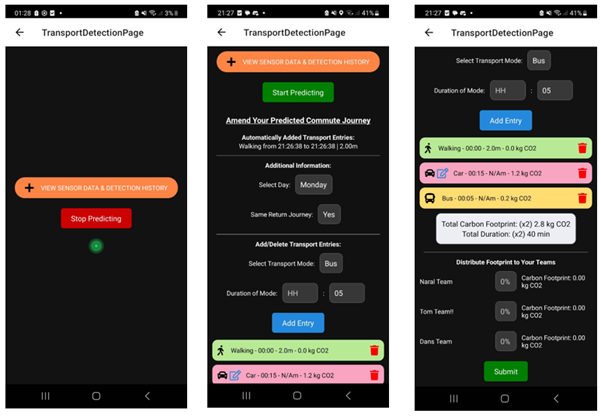
\includegraphics[width=\linewidth]{images/transport mode detection pages.png}
  \caption{Transport mode detection pages.}
  \label{fig:transportmodedetection}
\end{figure}

Due to the novelty of transport mode detection applications, users might find interacting with the Green-Workplace mobile application confusing. To address this, a help button is integrated to provide guidance and clarify the app's features, aligning with UH\#10 (Help and Documentation). To avoid overwhelming users, details such as sensor data and detection history are not displayed upfront, adhering to principles of user-friendly design by keeping the interface simple and focused on primary functions. The app has buttons to allow users to indicate the start and end of their commute, where visual cues such as an animated ripple effect and occasional toast notifications are displayed to reassure users that the app is actively working.

It's acknowledged that users can be in more than one team, and can talk with each team for a different length of time at their office, as a result there the application is designed to allow users to distribute their carbon footprint as a percentage. Before submission, the app verifies that all inputs meet the necessary criteria, such as ensuring the total carbon footprint distribution equals 100\%. This functionality is a practical application of UH\#9, aiding users in identifying, understanding, and correcting errors, thereby streamlining the process and enhancing user satisfaction. Hence, React Native was chosen due to the factors of performance, community support, and consistency in development experience, making it the more advantageous option for our mobile application needs.

\section{Frameworks and Technologies}
Multiple frameworks and technologies were analysed for both the web and mobile apps.

\subsection{Frontend}

For the development of the web app, the framework options considered were React JS, Vue.js, and Angular. For a web app like Green-Workplace, with its need for dynamic chat and dashboard visuals, React JS excels due to its Virtual DOM. This method updates only what's needed, avoiding extensive DOM changes and boosting performance. Unlike Vue's two-way binding that complicates large apps, or Angular's bulky framework slowing rapid updates, React's streamlined process is more efficient for fast-paced and interactive applications (cite). Additionally, React's component-based design is a key benefit, enabling reusable UI elements perfect for Green-Workplace's diverse features. This design supports the separate development of components like dashboard charts and modals, streamlining the codebase. In contrast, Angular's rigid structure and Vue's variable organization can complicate managing complex applications (cite). Finally, React's vast ecosystem and supportive community offer numerous libraries and tools, surpassing those available in Vue or Angular. Particularly, the react library MUI offers developers a suite of ready-to-use, visually appealing UI components such as dashboard charts and input boxes, which can help streamline UI development in Green-Workplace (cite). Hence, React JS was chosen due to its performance, development ease, and comprehensive library ecosystem aligning with the dynamic and visually intensive requirements of Green-Workplace.

For the Mobile app, React Native and Flutter were considered as there are they are the two most used among developers (cite). React Native provides near-native performance and has excellent access to native functionalities, which is crucial for leveraging GPS and motion sensor data for transport mode detection. Whilst Flutter also offers high performance and good access to native features, its interaction with native components can be less direct compared to React Native. In terms of community support, React Native has a well-established community offering a wealth of resources, libraries, and support, whereas Flutter's community is still maturing compared to it (cite). Moreover, choosing React JS for the web app logically extends to selecting React Native for mobile development, ensuring consistency across coding practices and reducing the learning curve for developers transitioning between web and mobile platforms. Hence, React Native was chosen due to the factors of performance, community support, and consistency in development experience, making it the more advantageous option for our mobile application needs.

\subsection{Backend}

The framework options for the backend that were considered were Node.js with Express, Spring Boot (Java), and ASP.NET (C\#). (need to finish)


\subsection{Database}
Green-Workplace chose to select from relational databases as it excels in managing structured data with complex relationships. This is crucial for storing and querying detailed employee data, their voting results for hybrid work schedules, and their carbon footprint records. Relational databases are also known for their strong emphasis on ACID (Atomicity, Consistency, Isolation, Durability) compliance, providing data integrity. Ensuring the accuracy and consistency of data is crucial, especially when dealing with sensitive employee data and carbon emission records (cite). Among the potential options for a relational database, Supabase (PostgreSQL) and MySQL were considered. Supabase, being a cloud-based implementation of PostgreSQL, offers advanced capabilities in handling complex queries, robust performance, and real-time functionalities. MySQL, while also a powerful RDBMS, is more traditional and may not offer the same level of sophistication in real-time data processing and advanced query optimisation as Supabase (cite).

(need to finish)

\subsection{Summary}

%==================================================================================================================================
\chapter{Implementation}

\section{Software Engineering Process}
notes: Version control and continuous integration
Issue management
Iterative Development / Agile
Agile manifesto
Code reviews
testing 
documentation
adds/not adds value


\section{Transport Mode Detection Page}

\subsection{Data Collection}

The data collection selection and methods were crucial to achieving high accuracy in transport mode detection while minimising battery consumption. 
Based on the findings in section 2.3.1, the application leveraged the accelerometer, gyroscope, and GPS as they represented the optimal combination of minimal yet diverse sensors, offering the highest accuracy for transport mode detection. The application employed a low sampling rate of 1 second for accelerometer and gyroscope logging. GPS logging utilised a slightly higher rate of 7 seconds, which finds the balance between battery efficiency as well as getting vital distance information for accurate transport detection and commuting carbon footprint.

The mobile application also implements an overlapping windowing technique in the data collection process to further increase accuracy and decrease battery usage. This approach involves collecting sensor data (accelerometer, gyroscope, and GPS) in fixed-size windows with a specified overlap between consecutive windows. Specifically, the application collects data in 42-second windows, with each window sharing a 50\% overlap with its predecessor. This means that new data is sent to the backend every 21 seconds, effectively doubling the resolution of the data collection phase without significantly increasing power consumption. The window overlap captures vital transitional moments, providing richer data for significantly more accurate transport mode classification (cite). 

(whilst distance gets accumulated in a window, distance also is tracked between sending to the backend (21 sec period - so that the transport mode detection would be assocated with that distance to accurately acculate carbon footprint.

\begin{figure}[ht]
  \centering
  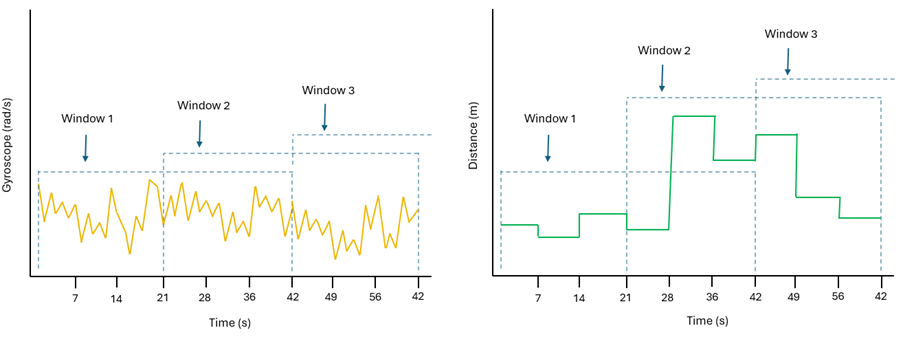
\includegraphics[width=\linewidth]{images/overlap windowing.png}
  \caption{Gyroscope and distance example for overlap windowing.}
  \label{fig:overlapWindowing}
\end{figure}


\subsection{Pre-processing}
One pre-processing step employed is noise filtering from discarding invalid GPS points due to smartphone with low signal, by only accepting high location accuracy collection. Another pre-processing step applied is taking magnitude values of both acceleration and gyroscope data. This conversion ensures the classifier's robustness against the influence of frequent changes in the phone's position and orientation, which focuses on the strength and direction of movement.

The magnitude of a vector \(\vec{a}\) representing either acceleration or gyroscope data is calculated as:
\begin{equation}
\text{Magnitude} = \sqrt{a_x^2 + a_y^2 + a_z^2}
\end{equation}
where \(a_x\), \(a_y\), and \(a_z\) are the x, y, and z components of the vector, respectively.

\subsection{Feature Extraction}
After pre-processing, the following features were extracted from accelerometer and gyroscope data as they have been proven to be successful in TMD according to section 2.3.1: minimum, maximum, mean, and standard deviation. Additionally, the distance calculated was calculated from the latitude and longitude readings from the GPS sensor.

The formula to calculate distance \(D\) between two points given their latitude and longitude is based on the Haversine formula (cite):
\begin{equation}
D = 2r \arcsin\left(\sqrt{\sin^2\left(\frac{\Delta \phi}{2}\right) + \cos(\phi_1) \cos(\phi_2) \sin^2\left(\frac{\Delta \lambda}{2}\right)}\right)
\end{equation}
where \(\phi_1\) and \(\phi_2\) are the latitudes of the two points in radians, \(\Delta \phi\) is the difference in latitudes, \(\Delta \lambda\) is the difference in longitudes in radians, and \(r\) is the radius of the Earth (approximately 6371 kilometers).

\subsection{Classification and Training}

A dataset of 5,000 data points across five transport mode categories (still, walking, bus, car, train) was collected from six participants (aged 22-65) who self-reported their transport modes. The Dataset was split 70/30 into training and testing sets and the data was evaluated using various algorithms to determine its accuracy in detecting transport modes.

\begin{table}[ht]
\centering
\begin{tabular}{|l|c|}
\hline
Classifier Algorithm             & Accuracy \\ \hline
Random Forest                    & 96\%     \\
DecisionTreeClassifier (CART)    & 92\%     \\
KNN                              & 84\%     \\
Naïve Bayes                      & 74\%     \\ \hline
\end{tabular}
\caption{Accuracy of Different Classifier Algorithms}
\label{tab:classifier_accuracy}
\end{table}

The Random forest algorithm provided the highest accuracy in Figure 6 and hence was chosen as the applications classifier model.

\subsection{Trip recognition algorithm}

A pivotal component of our transport mode detection application is the trip recognition algorithm. This algorithm plays a crucial role in determining the start and end times of a transport mode, based on a consecutive sequence of 20-second detections throughout the entire trip. This aggregation is crucial for understanding the trip's structure, including transitions between different transport modes and the duration and distance covered by each mode.

The trip recognition algorithm (see Appendix [5]) operates on a series of transport mode detections, each tagged with a timestamp and associated distance. Its primary objective is to aggregate these detections into meaningful segments, each corresponding to a continuous use of a single mode of transport, such as walking, driving a car, or riding a bus. Since the algorithm iterates through each detection exactly once in a single pass, its time complexity is O(n), where n represents the total number of detections within the dataset for a single trip. This linear time complexity makes the algorithm scalable to handle trips with a large number of detections without a significant increase in processing time.


\section{Google Maps API Page}

The Google Maps API Page is the web based solution for calculating a user’s carbon footprint. Google Maps API is a set of JavaScript classes that enable users to customise and embed Google Maps in their webpages. Whilst Google Maps API is a free service it imposes technical limits such as daily and per-second query caps, therefore it is imperative to opimise API usage to avoid exceeding these thresholds.

5.3.1 API Integration and Initial Setup

The integration process begins with the ‘useJSApiLoader’ hook, which is responsible for the asynchronous loading of the Google Maps JavaScript API. This step is essential for activating the map's rendering capabilities and accessing various mapping services. During this phase, the useJSApiLoader is configured with the API key and instructed to load specific libraries required by the application, notably the 'places' library. The application employs conditional rendering based on the 'isLoaded' state, to defer API requests until the API is fully loaded, thus averting potential errors.
 
5.3.2 Map Display and Functionality

Upon successful loading of the Google Maps API, the application presents an interactive map via the GoogleMap component. The application configures initial map settings that deactivates unnecessary controls like streetViewControl to streamline the user experience and minimise API usage. The user inputs for users entering their Home and Office Destination addresses incorporate the autocomplete functionality from the Places API, suggesting possible addresses in real-time, to streamline the address entry process. The Directions API plays a vital role in our application by processing user-provided details such as location, date, departure time, and chosen mode of transport to map out travel routes while also providing estimates of distance and journey duration. These estimates are integral to our carbon footprint assessment tool, where the distance data obtained from the Directions API is utilised within our algorithm to calculate CO2 emissions tailored to the selected mode of transport. Notably, for journeys involving multiple transit types—like bus, walking, and subway—the API delineates the distance covered by each mode, enabling our algorithm to deliver a more precise carbon footprint estimation.

Minimising API rate limits


\section{Team Chat Page}


\section{State management}


\section{Deployment}

------------------
What did you do to implement this idea, and what technical achievements did you make?
\section{Guidance}
You can't talk about everything. Cover the high level first, then cover important, relevant or impressive details.



\section{General points}

These points apply to the whole dissertation, not just this chapter.



\subsection{Figures}
\emph{Always} refer to figures included, like Figure \ref{fig:relu}, in the body of the text. Include full, explanatory captions and make sure the figures look good on the page.
You may include multiple figures in one float, as in Figure \ref{fig:synthetic}, using \texttt{subcaption}, which is enabled in the template.





\clearpage

\subsection{Equations}

Equations should be typeset correctly and precisely. Make sure you get parenthesis sizing correct, and punctuate equations correctly 
(the comma is important and goes \textit{inside} the equation block). Explain any symbols used clearly if not defined earlier. 

For example, we might define:
\begin{equation}
    \hat{f}(\xi) = \frac{1}{2}\left[ \int_{-\infty}^{\infty} f(x) e^{2\pi i x \xi} \right],
\end{equation}    
where $\hat{f}(\xi)$ is the Fourier transform of the time domain signal $f(x)$.

\subsection{Algorithms}
Algorithms can be set using \texttt{algorithm2e}, as in Algorithm \ref{alg:metropolis}.

% NOTE: line ends are denoted by \; in algorithm2e
\begin{algorithm}
    \DontPrintSemicolon
    \KwData{$f_X(x)$, a probability density function returing the density at $x$.\; $\sigma$ a standard deviation specifying the spread of the proposal distribution.\;
    $x_0$, an initial starting condition.}
    \KwResult{$s=[x_1, x_2, \dots, x_n]$, $n$ samples approximately drawn from a distribution with PDF $f_X(x)$.}
    \Begin{
        $s \longleftarrow []$\;
        $p \longleftarrow f_X(x)$\;
        $i \longleftarrow 0$\;
        \While{$i < n$}
        {
            $x^\prime \longleftarrow \mathcal{N}(x, \sigma^2)$\;
            $p^\prime \longleftarrow f_X(x^\prime)$\;
            $a \longleftarrow \frac{p^\prime}{p}$\;
            $r \longleftarrow U(0,1)$\;
            \If{$r<a$}
            {
                $x \longleftarrow x^\prime$\;
                $p \longleftarrow f_X(x)$\;
                $i \longleftarrow i+1$\;
                append $x$ to $s$\;
            }
        }
    }
    
\caption{The Metropolis-Hastings MCMC algorithm for drawing samples from arbitrary probability distributions, 
specialised for normal proposal distributions $q(x^\prime|x) = \mathcal{N}(x, \sigma^2)$. The symmetry of the normal distribution means the acceptance rule takes the simplified form.}\label{alg:metropolis}
\end{algorithm}

\subsection{Tables}

If you need to include tables, like Table \ref{tab:operators}, use a tool like https://www.tablesgenerator.com/ to generate the table as it is
extremely tedious otherwise. 

\begin{table}[]
    \caption{The standard table of operators in Python, along with their functional equivalents from the \texttt{operator} package. Note that table
    captions go above the table, not below. Do not add additional rules/lines to tables. }\label{tab:operators}
    %\tt 
    \rowcolors{2}{}{gray!3}
    \begin{tabular}{@{}lll@{}}
    %\toprule
    \textbf{Operation}    & \textbf{Syntax}                & \textbf{Function}                            \\ %\midrule % optional rule for header
    Addition              & \texttt{a + b}                          & \texttt{add(a, b)}                                    \\
    Concatenation         & \texttt{seq1 + seq2}                    & \texttt{concat(seq1, seq2)}                           \\
    Containment Test      & \texttt{obj in seq}                     & \texttt{contains(seq, obj)}                           \\
    Division              & \texttt{a / b}                          & \texttt{div(a, b) }  \\
    Division              & \texttt{a / b}                          & \texttt{truediv(a, b) } \\
    Division              & \texttt{a // b}                         & \texttt{floordiv(a, b)}                               \\
    Bitwise And           & \texttt{a \& b}                         & \texttt{and\_(a, b)}                                  \\
    Bitwise Exclusive Or  & \texttt{a \textasciicircum b}           & \texttt{xor(a, b)}                                    \\
    Bitwise Inversion     & \texttt{$\sim$a}                        & \texttt{invert(a)}                                    \\
    Bitwise Or            & \texttt{a | b}                          & \texttt{or\_(a, b)}                                   \\
    Exponentiation        & \texttt{a ** b}                         & \texttt{pow(a, b)}                                    \\
    Identity              & \texttt{a is b}                         & \texttt{is\_(a, b)}                                   \\
    Identity              & \texttt{a is not b}                     & \texttt{is\_not(a, b)}                                \\
    Indexed Assignment    & \texttt{obj{[}k{]} = v}                 & \texttt{setitem(obj, k, v)}                           \\
    Indexed Deletion      & \texttt{del obj{[}k{]}}                 & \texttt{delitem(obj, k)}                              \\
    Indexing              & \texttt{obj{[}k{]}}                     & \texttt{getitem(obj, k)}                              \\
    Left Shift            & \texttt{a \textless{}\textless b}       & \texttt{lshift(a, b)}                                 \\
    Modulo                & \texttt{a \% b}                         & \texttt{mod(a, b)}                                    \\
    Multiplication        & \texttt{a * b}                          & \texttt{mul(a, b)}                                    \\
    Negation (Arithmetic) & \texttt{- a}                            & \texttt{neg(a)}                                       \\
    Negation (Logical)    & \texttt{not a}                          & \texttt{not\_(a)}                                     \\
    Positive              & \texttt{+ a}                            & \texttt{pos(a)}                                       \\
    Right Shift           & \texttt{a \textgreater{}\textgreater b} & \texttt{rshift(a, b)}                                 \\
    Sequence Repetition   & \texttt{seq * i}                        & \texttt{repeat(seq, i)}                               \\
    Slice Assignment      & \texttt{seq{[}i:j{]} = values}          & \texttt{setitem(seq, slice(i, j), values)}            \\
    Slice Deletion        & \texttt{del seq{[}i:j{]}}               & \texttt{delitem(seq, slice(i, j))}                    \\
    Slicing               & \texttt{seq{[}i:j{]}}                   & \texttt{getitem(seq, slice(i, j))}                    \\
    String Formatting     & \texttt{s \% obj}                       & \texttt{mod(s, obj)}                                  \\
    Subtraction           & \texttt{a - b}                          & \texttt{sub(a, b)}                                    \\
    Truth Test            & \texttt{obj}                            & \texttt{truth(obj)}                                   \\
    Ordering              & \texttt{a \textless b}                  & \texttt{lt(a, b)}                                     \\
    Ordering              & \texttt{a \textless{}= b}               & \texttt{le(a, b)}                                     \\
    % \bottomrule
    \end{tabular}
    \end{table}
\subsection{Code}

Avoid putting large blocks of code in the report (more than a page in one block, for example). Use syntax highlighting if possible, as in Listing \ref{lst:callahan}.

\begin{lstlisting}[language=python, float, caption={The algorithm for packing the $3\times 3$ outer-totalistic binary CA successor rule into a 
    $16\times 16\times 16\times 16$ 4 bit lookup table, running an equivalent, notionally 16-state $2\times 2$ CA.}, label=lst:callahan]
    def create_callahan_table(rule="b3s23"):
        """Generate the lookup table for the cells."""        
        s_table = np.zeros((16, 16, 16, 16), dtype=np.uint8)
        birth, survive = parse_rule(rule)

        # generate all 16 bit strings
        for iv in range(65536):
            bv = [(iv >> z) & 1 for z in range(16)]
            a, b, c, d, e, f, g, h, i, j, k, l, m, n, o, p = bv

            # compute next state of the inner 2x2
            nw = apply_rule(f, a, b, c, e, g, i, j, k)
            ne = apply_rule(g, b, c, d, f, h, j, k, l)
            sw = apply_rule(j, e, f, g, i, k, m, n, o)
            se = apply_rule(k, f, g, h, j, l, n, o, p)

            # compute the index of this 4x4
            nw_code = a | (b << 1) | (e << 2) | (f << 3)
            ne_code = c | (d << 1) | (g << 2) | (h << 3)
            sw_code = i | (j << 1) | (m << 2) | (n << 3)
            se_code = k | (l << 1) | (o << 2) | (p << 3)

            # compute the state for the 2x2
            next_code = nw | (ne << 1) | (sw << 2) | (se << 3)

            # get the 4x4 index, and write into the table
            s_table[nw_code, ne_code, sw_code, se_code] = next_code

        return s_table

\end{lstlisting}

%==================================================================================================================================
\chapter{Evaluation} 
How good is your solution? How well did you solve the general problem, and what evidence do you have to support that?

\section{Guidance}
\begin{itemize}
    \item
        Ask specific questions that address the general problem.
    \item
        Answer them with precise evidence (graphs, numbers, statistical
        analysis, qualitative analysis).
    \item
        Be fair and be scientific.
    \item
        The key thing is to show that you know how to evaluate your work, not
        that your work is the most amazing product ever.
\end{itemize}

\section{Evidence}
Make sure you present your evidence well. Use appropriate visualisations, reporting techniques and statistical analysis, as appropriate.

If you visualise, follow the basic rules, as illustrated in Figure \ref{fig:boxplot}:
\begin{itemize}
\item Label everything correctly (axis, title, units).
\item Caption thoroughly.
\item Reference in text.
\item \textbf{Include appropriate display of uncertainty (e.g. error bars, Box plot)}
\item Minimize clutter.
\end{itemize}

See the file \texttt{guide\_to\_visualising.pdf} for further information and guidance.

\begin{figure}
    \centering
    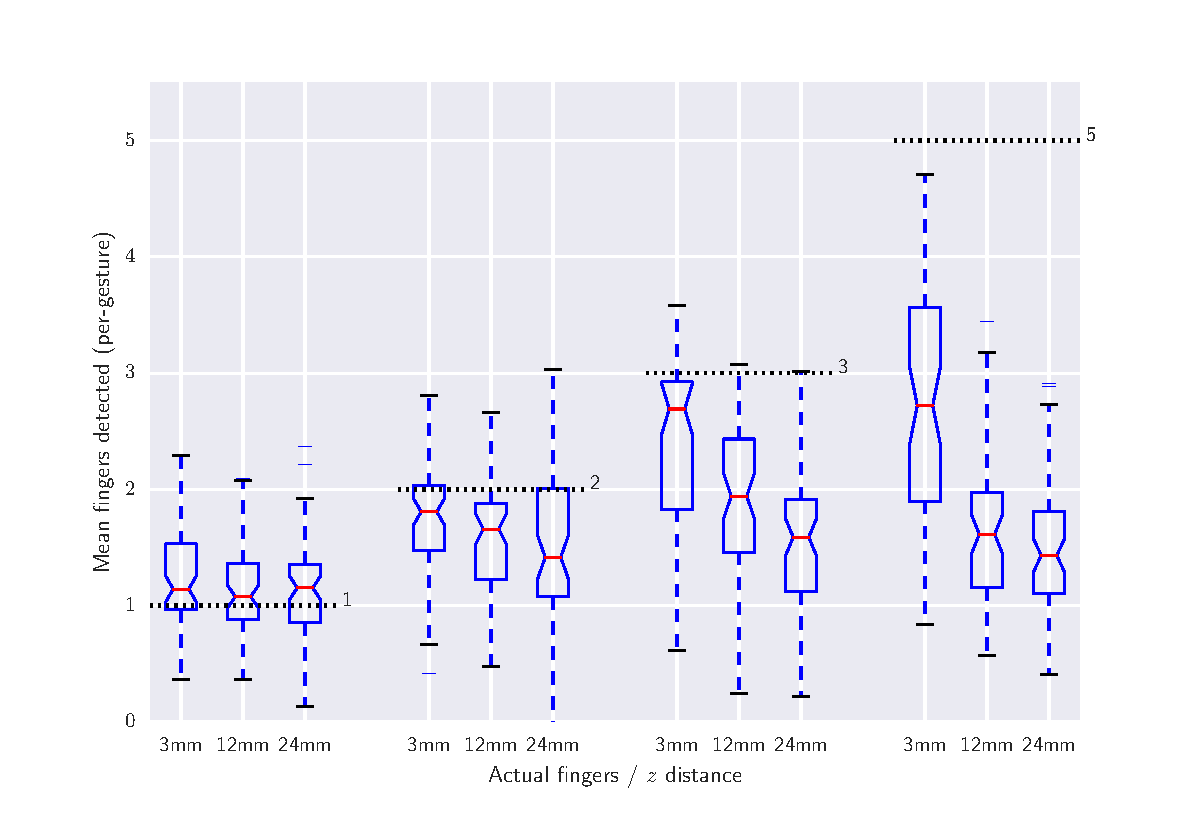
\includegraphics[width=1.0\linewidth]{images/boxplot_finger_distance.pdf}    

    \caption{Average number of fingers detected by the touch sensor at different heights above the surface, averaged over all gestures. Dashed lines indicate
    the true number of fingers present. The Box plots include bootstrapped uncertainty notches for the median. It is clear that the device is biased toward 
    undercounting fingers, particularly at higher $z$ distances.
    }

    % use the notation fig:name to cross reference a figure
    \label{fig:boxplot} 
\end{figure}


%==================================================================================================================================
\chapter{Conclusion}    
Summarise the whole project for a lazy reader who didn't read the rest (e.g. a prize-awarding committee).
\section{Guidance}
\begin{itemize}
    \item
        Summarise briefly and fairly.
    \item
        You should be addressing the general problem you introduced in the
        Introduction.        
    \item
        Include summary of concrete results (``the new compiler ran 2x
        faster'')
    \item
        Indicate what future work could be done, but remember: \textbf{you
        won't get credit for things you haven't done}.
\end{itemize}

%==================================================================================================================================
%
% 
%==================================================================================================================================
%  APPENDICES  

\begin{appendices}

\chapter{Appendices}

Typical inclusions in the appendices are:

\begin{itemize}
\item
  Copies of ethics approvals (required if obtained)
\item
  Copies of questionnaires etc. used to gather data from subjects.
\item
  Extensive tables or figures that are too bulky to fit in the main body of
  the report, particularly ones that are repetitive and summarised in the body.

\item Outline of the source code (e.g. directory structure), or other architecture documentation like class diagrams.

\item User manuals, and any guides to starting/running the software.

\end{itemize}

\textbf{Don't include your source code in the appendices}. It will be
submitted separately.

\end{appendices}



\begin{figure}
    \centering
    \begin{subfigure}[b]{0.45\textwidth}
        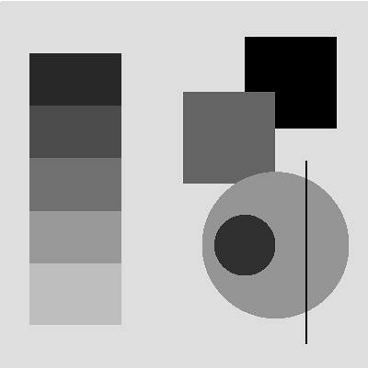
\includegraphics[width=\textwidth]{images/synthetic.png}
        \caption{Synthetic image, black on white.}
        \label{fig:syn1}
    \end{subfigure}
    ~ %add desired spacing between images, e. g. ~, \quad, \qquad, \hfill etc. 
      %(or a blank line to force the subfigure onto a new line)
    \begin{subfigure}[b]{0.45\textwidth}
        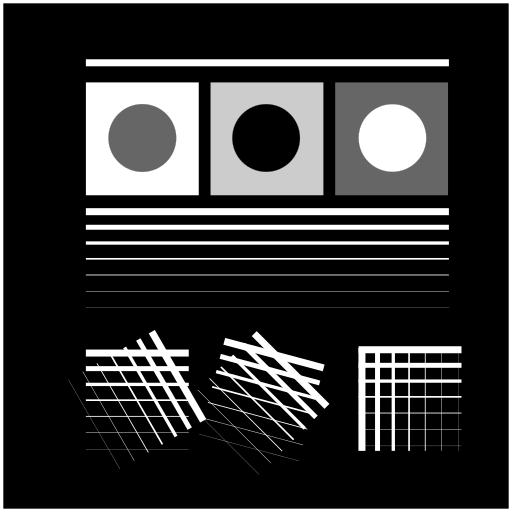
\includegraphics[width=\textwidth]{images/synthetic_2.png}
        \caption{Synthetic image, white on black.}
        \label{fig:syn2}
    \end{subfigure}
    ~ %add desired spacing between images, e. g. ~, \quad, \qquad, \hfill etc. 
    %(or a blank line to force the subfigure onto a new line)    
    \caption{Synthetic test images for edge detection algorithms. \subref{fig:syn1} shows various gray levels that require an adaptive algorithm. \subref{fig:syn2}
    shows more challenging edge detection tests that have crossing lines. Fusing these into full segments typically requires algorithms like the Hough transform.
    This is an example of using subfigures, with \texttt{subref}s in the caption.
    }\label{fig:synthetic}
\end{figure}



% Figures are important. Use them well.
\begin{figure}
    \centering
    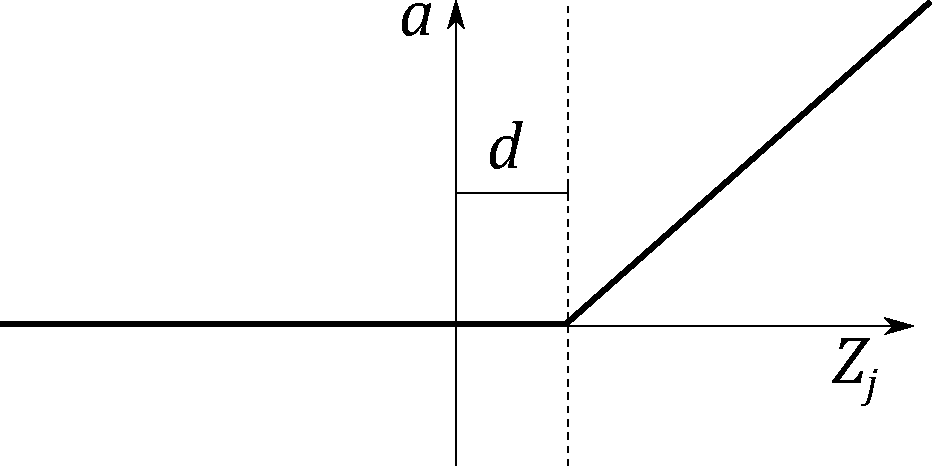
\includegraphics[width=0.5\linewidth]{images/relu.pdf}    

    \caption{In figure captions, explain what the reader is looking at: ``A schematic of the rectifying linear unit, where $a$ is the output amplitude,
    $d$ is a configurable dead-zone, and $Z_j$ is the input signal'', as well as why the reader is looking at this: 
    ``It is notable that there is no activation \emph{at all} below 0, which explains our initial results.'' 
    \textbf{Use vector image formats (.pdf) where possible}. Size figures appropriately, and do not make them over-large or too small to read.
    }

    % use the notation fig:name to cross reference a figure
    \label{fig:relu} 
\end{figure}

%==================================================================================================================================
%   BIBLIOGRAPHY   

% The bibliography style is abbrvnat
% The bibliography always appears last, after the appendices.

\bibliographystyle{abbrvnat}

\bibliography{l4proj}

\end{document}
